\documentclass{beamer}
\usepackage{beamerthemeshadow}
\usepackage{graphicx}
\usepackage{color}
\usepackage[utf8]{inputenc}
\usepackage{hyperref}
\usepackage[flushleft]{threeparttable}
\usepackage{csquotes}
\usepackage[english,serbian]{babel}
\usepackage{tabularx}
\usepackage{adjustbox}
\usetheme{Hannover}
\usecolortheme{wolverine}
% \setbeamertemplate{headline}{}
\setbeamersize{sidebar width left=0pt}
\setbeamertemplate{sidebar left}{}
% \definecolor{beamer@green}{rgb}{0.5, 2, 0.5}
% \setbeamercolor{structure}{fg=beamer@green}

\usepackage{listings}
\usepackage{verbatim}
% \usepackage{pseudocode}
\usepackage{algorithm}
\usepackage{algorithmic}
\usepackage{tabularx}
\usepackage{adjustbox}
\floatname{algorithm}{Algoritam}
% \newcommand\newf{\fontsize{9}{7.2}\selectfont}

\def\dJ{{\fontencoding{T1}\selectfont\dj}}
\def\Dj{{\fontencoding{T1}\selectfont\DJ}}

% my commands
\newcommand{\q}[1]{``#1''}  %use this command for quoting
\newcommand{\s}[0]{\textit{s}} %use this for italic s
\newcommand{\sstar}[0]{$\textit{s}^*$}
\newcommand{\squote}[0]{$\textit{s}^\prime$}
\renewcommand{\S}[0]{$\mathcal{S}$} %use this for instead of $\mathcal{S}$
\newcommand{\Sstar}[0]{$\mathcal{S}^{*}$}
\newcommand{\eng}[1]{(\textit{eng.} #1)}
\newcommand{\lokalna}[0]{\small{\texttt{LokalnaPretraga}}}
\newcommand{\kriterijum}[0]{\small{\texttt{KriterijumPrihvatanja}}}
\newcommand{\generisi}[0]{\small{\texttt{GenerišiPočetnoRešenje}}}
\newcommand{\perturbacija}[0]{\small{\texttt{Perturbacija}}}

\begin{document}
\title{Iterativna lokalna pretraga}
\author[]{Aleksa Voštić, Lazar Perišić,\\ Anđela Križan, Anđela Janošević}
\institute{Matematički fakultet\\Univerzitet u Beogradu}
\date{
	\footnotesize{Beograd, 2020.}	
}

\begin{frame}
	\thispagestyle{empty}
	\titlepage
\end{frame}

%-----------------------------------------------------------------

%-----------------------------------------------------------------

\section*{Uvod}
\begin{frame}[fragile]
  \frametitle{Uvod}
  % \newf
	\begin{itemize}
		\item Metaheurističke metode za rešavanje teških optimizacionih problema
		\item Prilikom dizajniranja metaheuristike, poželjno je da bude jednostavna, efikasna, opšte namene
		\item Idealan slučaj je kada se metaheuristika može koristiti bez ikakvog znanja o zavisnosti od problema
		\item Znanje specifično za problem mora biti inkorporirano u metaheuristiku da bi se dostiglo vrhunsko stanje
		\item Pokušavamo da dekomponujemo metaheuristički algoritam na nekoliko delova:
		\begin{itemize}
			\item potpuno opšti namenski deo
			\item svako znanje specifično za problem ugrađeno u metaheuristiku bilo bi odvojeno u drugi deo
		\end{itemize}
	\end{itemize}

\end{frame}

\begin{frame}[fragile]
	\frametitle{Uvod}
	\begin{itemize}
		\item Iterativna lokalna pretraga pruža jednostavan način da se zadovolje svi ovi zahtevi
		\item Suština iterativne lokalne pretrage je da se izbegne zaglavljivanje u lokalnom minimumu tako što u više iteracija primenjuje lokalnu pretragu na novo generisano početno rešenje
		\item Ova ideja ima dugu istoriju, a njeno ponovno otkriće od strane mnogih autora dovelo je do mnogo različitih imena za iterativnu lokalnu pretragu poput iterativnog spusta, Markovljevi lanci velikog koraka, iterativni Lin-Kernigan, lančana lokalna optimizacija...
	\end{itemize}

\end{frame}
%------------------------------------------------------------------------

\section{Ideja iza iterativne lokalne pretrage}
\begin{frame}
	\frametitle{Ideja iza iterativne lokalne pretrage} 
  \begin{itemize}
    \item Koristimo samo podskup rešenja, dobijen od lokalne pretrage
    \begin{center}
      \begin{minipage}{1\linewidth}
        \begin{algorithm}[H]
      \caption{Iterativna lokalna pretraga}
      \label{alg:1}
      \begin{algorithmic}
      \STATE $\textit{s}_0$ = \generisi{}()
      \STATE \sstar{} = \lokalna{}($\textit{s}_0$)
      \REPEAT
      \STATE \squote{} = \perturbacija{}(\sstar{}, \textit{istorija})
      \STATE $\textit{s}^{*\prime}$ = \lokalna{}(\squote{})
      \STATE \sstar{} = \kriterijum{}(\sstar{}, $\textit{s}^{*\prime}$, \textit{istorija})
      \UNTIL \textsc{nije zadovoljen uslov zaustavljanja}\footnotemark
      \RETURN \textsc{najbolje rešenje}
      \end{algorithmic}
      \end{algorithm}
    \end{minipage}
    \end{center}
  \end{itemize}
\end{frame}
%-----------------------------------------------------------------------

% \section{Implementacija iterativne lokalne pretrage}
\begin{frame}[fragile]\frametitle{Ideja iza iterativne lokalne pretrage}
  \begin{figure}[h!]
    \centering
    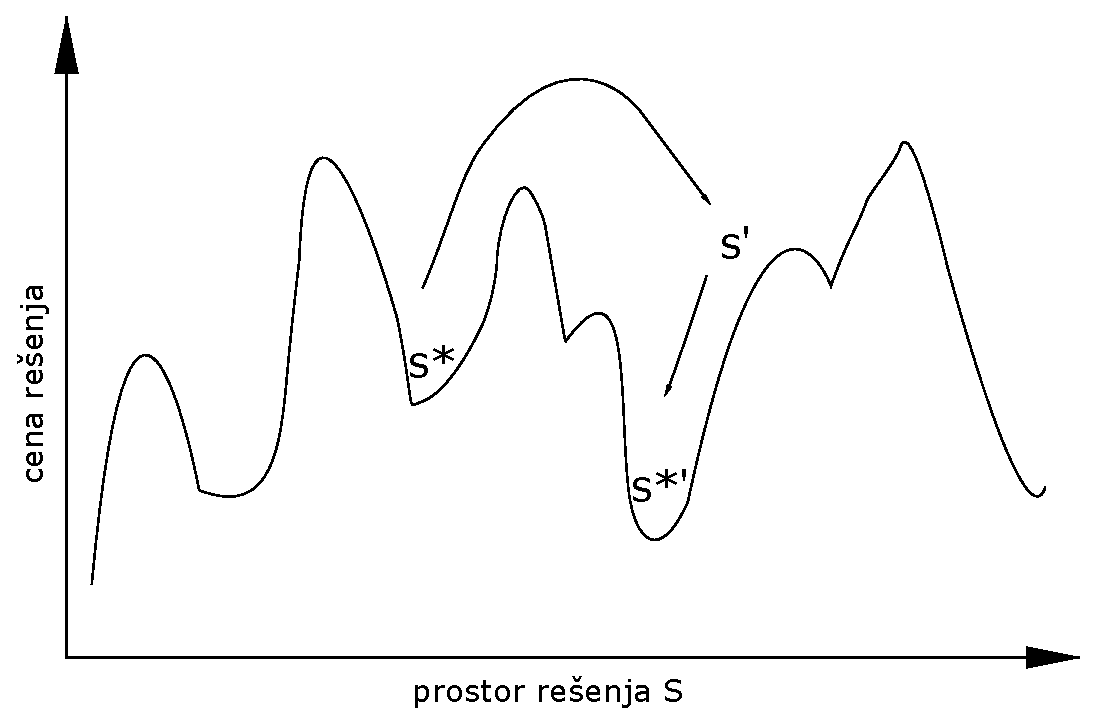
\includegraphics[width=0.5\textwidth]{slika.eps}
    \begin{itemize}
      \item Početno rešenje
      \item Lokalna pretraga
      \item Perturbacija
      \item Kriterijum prihvatanja
    \end{itemize}
  \end{figure}
\end{frame}

\section{Implementacija iterativne lokalne pretrage}
\subsection{Početno rešenje i Perturbacija}
\begin{frame}[fragile]\frametitle{Početno rešenje i Perturbacija}
  Početno rešenje
  \begin{itemize}
    \item Najmanje uticaja na algoritam
    \item Metoda slučajnog izbora
    \item Metoda pohlepne heuristike
  \end{itemize}
  Perturbacija
  \begin{itemize}
    \item Veoma važna komponenta algoritma
    \item Služe da se pobegne od lokalnog optimuma
    \item Snaga perturbacije
    \item Adaptivne perturbacije
  \end{itemize}
	\subsection{Perturbacija}

\end{frame}

% \subsection{Perturbacija}
% \begin{frame}[fragile]\frametitle{Perturbacija}

% \end{frame}


\subsection{Kriterijum prihvatanja i Lokalna pretraga}
\begin{frame}[fragile]\frametitle{Kriterijum prihvatanja i Lokalna pretraga}
	Kriterijum prihvatanja
  \begin{itemize}
    \item Prihvati svako rešenje
    \item Prihvati samo bolje rešenje
  \end{itemize}
  Lokalna pretraga
  \begin{itemize}
    \item Poznavanje implementacije može nam pomoći prilikom optimizacije ILS
    \item Najčešće važi da što je bolja pretraga to je bolji ILS
    \item Mnogo različitih algoritama se koristi kao lokalna pretraga
  \end{itemize}
\end{frame}

% \subsection{Lokalna pretraga}
% \begin{frame}[fragile]\frametitle{Lokalna pretraga}

% \end{frame}
\section{Primene iterativne lokalne pretrage}
\begin{frame}[fragile]\frametitle{Primene iterativne lokalne pretrage}
Algoritmi iterativne lokalne pretrage su uspešno primenjeni u raznim kombinatornim optimizacionim problemima. Neki od njih su:
\begin{itemize}
   \item \textbf{problem trgovačkog putnika} \eng{travelling salesman problem} tj. TSP
  \item \textbf{problem rasporeda na jednoj mašini pomoću ukupnog kašnjenja sa težinskim koeficijentima} \eng{single machine total weighted tardiness problem} tj. SMTWTP
  \item \textbf{problem rasporeda n proizvoda na m mašina} \eng{flow shop problem} tj. FSP
  \item \textbf{problem raspoređivanja poslova} \eng{job shop scheduling problem} tj. JSSP
\end{itemize}

\end{frame}

\subsection{Problem trgovačkog putnika}
\begin{frame}[fragile]\frametitle{Problem trgovačkog putnika}
%smanji reci
Za dat skup gradova i cena putovanja između njih, naći najjeftiniju rutu koja obilazi svaki grad tačno jednom, i vraća se u početni grad.
\begin{itemize}
  \item Verovatno najpoznatiji kombinatorni optimizacijski problem
  \item Služi za testiranje izrade novih ideja algoritama, dobre performanse na ovom problemu su dokaz vrednosti takvih ideja
  \item Baum je prvi testirao svoju metodu ponovljenog spusta na TSP, koristio je tehniku 2-opt kao heuristiku, nasumične 3-promene kao perturbacije, nezadovoljavajući rezultati
  \item Algoritam Large-step Markov chain(tj. LSMC) doneo poboljšanja, korišćeno simulirano kaljenje kao optimizacija i Lin-Kernighan (tj. LK) heuristika. Autori Martin, Otto i Felten
\end{itemize}
\end{frame}

%drugi slajd:
\begin{frame}[fragile]\frametitle{Problem trgovačkog putnika}
\begin{itemize}
  \item  D.S.Johnson koristio LK kao lokalnu pretragu, naziv algoritma "iterated Lin-Kernighan" 
  \item Applegate, Bixby, Chivatal i Cook implementirali lančani LK, vršili testove na instancama do 25 miliona gradova, zaključili su da najbolje performanse daje između ostalog i pohlepna heuristika
  \item Katayama i Narisha u svoj algoritam uveli su novi mehanizam perturbacije-genetska transformacija koji koristi 2 obilaska
  \item Iterativni LK koji koristi genetsku transformaciju umesto standardnog dvostrukog mosta pokazao je bolje rezultate
\end{itemize}
\end{frame}

\subsection{Problemi raspoređivanja}
\subsubsection{Single machine total weighted tardiness problem}
\begin{frame}[fragile]\frametitle{Single machine total weighted tardiness problem}
Problem se sastoji od skupa nezavisnih poslova sa različitim vremenima obrade, težinama (cenama), kao i rokovima do kad poslovi moraju biti završeni predviđenim da se obrađuju na jednoj datoj mašini. \\
\begin{itemize}
  \item Početno rešenje se može generisati pomoću raznih heuristika konstrukcija (EDD, MDD, AU).
  \item Perturbacija se sastoji od niza proizvoljnih nezavisnih poteza razmene: posao na poziciji \textit{i} se razmenjuje sa poslom na poziciji \textit{j}. Razmena \textit{i}, \textit{j} se ne preklapa sa razmenom \textit{k}, \textit{l} ukoliko važi:\\ min\{\textit{i}, \textit{j}\} $\geq$ max\{\textit{k}, \textit{l}\} ili obrnuto.
  \item Kriterijum prihvatanja: backtrack korak, svako novo najbolje lokalno stanje se prihvata, algoritam se restartuje sa najboljim pronađenim rešenjem.
\end{itemize}
\end{frame}

\subsubsection{Flow shop problem}
\begin{frame}[fragile]\frametitle{Flow shop problem}
\begin{figure}[h!]
  \centering
  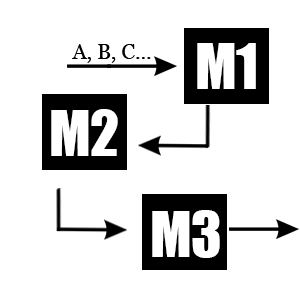
\includegraphics[width=0.2\textwidth]{flowshop.png}
  \label{figure:fsp}
\end{figure}
\begin{itemize}
  \item Početno rešenje se generiše uz pomoć NEH heuristike.
  \item Perturbacija se generiše pomoću dva različita tipa poteza: \\
	\begin{itemize}
 		 \item \begin{figure}[h!]
 			 \centering
  			 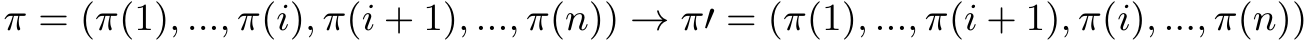
\includegraphics[width=0.8\textwidth]{f1.png}
		            \label{figure:f1}
			  \end{figure}
		\item \begin{figure}[h!]
 			 \centering
  			 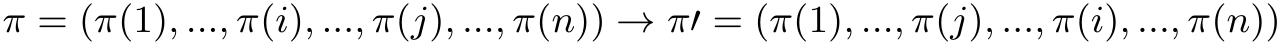
\includegraphics[width=0.8\textwidth]{f2.png}
		            \label{figure:f2}
			  \end{figure}
	\end{itemize}
  \item Kriterijum prihvatanja: može se uvek birati stanje koje je bolje i da se ono zadrži, ili napredniji slučaj koji analizira novo stanje i prihvata ga korišćenjem odgovarajuće verovatnoće.
\end{itemize}
\end{frame}

\section{Efektivnost i efikasnost ILS algoritma}
\begin{frame}[fragile]\frametitle{Efektivnost i efikasnost ILS algoritma}

\begin{gather*}
\textrm{\% Vremenskog uvećanja u odnosu na optimalno rešenje} = \\\frac{Alg_{rez} - Opt_{rez}}{Opt_{rez}} \cdot100
\end{gather*}
\begin{table}[H]
  \label{tab:alg}
  \begin{center}
      \begin{adjustbox}{max width=0.5\linewidth,center}
   \begin{tabular}{c c c c c c c} 
   \hline
   Problem & SAOP & SPIRIT & GAChen & GAMIT & ILS &\\ [0.5ex] 
   \hline\hline
   20x5 & 1.39 ($\leq$0.5) & 5.22 ($\leq$0.5) & 3.82 ($\leq$0.5) & 4.21 ($\leq$0.5) & 0.24 (4.01) &\\ [1ex]
   \hline
   20x10 & 2.66 ($\leq$0.5) & 5.86 ($\leq$0.5) & 4.89 ($\leq$0.5) & 5.40 ($\leq$0.5) & 0.77 (4.09) &\\ [1ex]
   \hline
   20x20 & 2.31 ($\leq$0.5) & 4.58 ($\leq$0.5) & 4.17 (0.60) & 4.53 ($\leq$0.5) & 0.85 (4.63) &\\ [1ex]
   \hline
   50x5 & 0.69 ($\leq$0.5) & 2.03 ($\leq$0.5) & 2.09 (0.77) & 3.11 ($\leq$0.5) & 0.12 (6.38) &\\ [1ex]
   \hline
   50x10 & 4.25 (0.60) & 5.88 (0.52) & 6.60 (1.00) & 8.38 (0.52) & 2.01 (9.94) &\\ [1ex] 
   \hline
   50x20 & 5.13 (1.04) & 7.21 (0.97) & 8.03 (1.45) & 10.65 (0.96) & 3.29 (11.82) &\\ [1ex] 
   \hline
   100x5 & 0.40 (0.60) & 1.06 (0.53) & 1.32 (1.79) & 5.41 (0.52) & 0.11 (15.31) &\\ [1ex] 
   \hline
   100x10 & 1.88 (1.10) & 5.07 (1.03) & 3.75 (2.26) & 12.05 (1.02) & 0.66 (18.79) &\\ [1ex] 
   \hline
   100x20 & 5.21 (2.09) & 10.15 (2.00) & 7.94 (3.24) &18.24 (1.99) & 3.17 (24.04) &\\ [1ex] 
   \hline
   200x10 & 1.56 (2.29) & 9.03 (2.25) & 2.70 (5.97) & 7.52 (2.20) & 0.49 (33.73) &\\ [1ex] 
   \hline
   200x20 & 4.83 (4.59) & 16.17 (4.51) & 7.07 (8.18) & 15.35 (4.50) & 2.74 (41.80) &\\ [1ex] 
   \hline
   500x20 & 3.40 (39.48) & 13.57 (39.70) & 4.61 (55.30) & 12.17 (37.82) & 1.29 (192.03) &\\ [1ex] 
   \hline
   \hline
   Average & 2.81 (4.42) & 7.15 (4.38) & 4.75 (6.77) & 8.92 (4.21) & 1.31 (30.55) &\\ [1ex] 
   \end{tabular}
  \end{adjustbox}
  \end{center}
  \end{table}
\end{frame}

\section{Zaključak}
\begin{frame}[fragile]\frametitle{Zaključak}
	\begin{itemize}
		\item ILS poseduje mnoge poželjne karakteristike metaheuristike: jednostavan je, lagan za implementaciju, robustan i veoma efikasan
		\item Suštinska ideja ILS-a leži u fokusiranju pretraživanja ne na celokupnom prostoru rešenja, već na manjem potprostoru koji je definisan rešenjima koja su lokalno optimalna za datu optimizaciju
		\item  Koliko će se ovaj pristup pokazati efikasnim, uglavnom zavisi od izbora lokalne pretrage, perturbacija i kriterijuma prihvatanja
		\item Zbog svojih karakteristika verujemo da je ILS obećavajući i moćan algoritam za rešavanje stvarnih kompleksnih problema
	\end{itemize}

\end{frame}

\begin{frame}[fragile]\frametitle{Literatura}
	\thispagestyle{empty}
  \begin{thebibliography}{10}
    \bibitem{Handbook of metaheuristics}
    \alert{Gendreau, Michel and Potvin, Jean-Yves}
    \newblock  {Handbook of metaheuristics}
    \newblock {\em 2010}.
    
    \bibitem{beginnersIntroduction}
    \alert{R. Lourenço, Helena and Martin, Olivier and Stützle, Thomas}
    \newblock {A beginner's introduction to Iterated Local Search}
    \newblock {\em 2001}.

    \bibitem{designOfIteratedLocalSearchAlgorithms}
    \alert{den Besten,  Matthijs and Stützle, Thomas and Dorigo, Marco}
    \newblock {Design of Iterated Local Search Algorithms}
    \newblock {\em 2001}.

    \bibitem{jobShopScheduling}
    \alert{Helena R. Lourenço}
    \newblock {Job-shop scheduling: Computational study of local search and large-step optimization methods}
    \newblock {\em 1995}.
    \end{thebibliography}
\end{frame}


\end{document}
